% Báo cáo seminar HFR-MKGC (AAAI 2026).
% Biên dịch: tectonic report.tex   (hoặc xelatex report.tex, chạy 2 lần)
\documentclass[11pt,a4paper]{article}

\usepackage{fontspec}
\setmainfont{Times New Roman}
\usepackage{polyglossia}
\setdefaultlanguage{vietnamese}
\usepackage[margin=2.3cm]{geometry}
\usepackage{amsmath,amssymb}
\usepackage{graphicx}
\usepackage{booktabs}
\usepackage{multirow}
\usepackage{array}
\usepackage{caption}
\usepackage{enumitem}
\usepackage{xcolor}
\usepackage{microtype}
\usepackage{float}
\PassOptionsToPackage{hyphens}{url}
\usepackage[hidelinks]{hyperref}

\graphicspath{{paper-vi/figures/}}
\captionsetup{font=small,labelfont=bf}
\setlist{nosep,leftmargin=*}
\setlength{\parskip}{3pt}
\renewcommand{\arraystretch}{1.15}

\newcommand{\Hj}{\mathbf{H}_{\mathrm{joint}}}
\newcommand{\Tj}{\mathbf{T}_{\mathrm{joint}}}
\newcommand{\Tjt}{\tilde{\mathbf{T}}_{\mathrm{joint}}}
\newcommand{\Hjt}{\tilde{\mathbf{H}}_{\mathrm{joint}}}
\newcommand{\Tm}{\mathbf{T}_{\mathrm{MLLM}}}
\renewcommand{\Re}{\operatorname{Re}}
\renewcommand{\Im}{\operatorname{Im}}
\newcommand{\score}{\mathrm{score}}
\newcommand{\Prom}{\mathrm{Prom}}
\newcommand{\Ent}[1]{\textit{#1}}

\title{\textbf{BÁO CÁO SEMINAR}\\[6pt]
\Large HFR-MKGC: Hierarchical Fusion Reasoning with MLLMs\\for Multi-modal Knowledge Graph Completion\\[4pt]
\large\textit{Suy luận hợp nhất phân cấp với MLLM cho bài toán hoàn thiện đồ thị tri thức đa phương thức}}

\author{
\begin{tabular}{ll}
25C11050 & Nguyễn Đình Lộc\\
25C15003 & Ngô Trương Minh Đạt
\end{tabular}\\[8pt]
\small Bài báo trình bày: D. Wang \textit{et al.}, AAAI 2026, vol.~40, tr.~15815--15823~\cite{hfr}.
}
\date{}

\begin{document}
\maketitle

\noindent\textbf{Ghi chú về trích dẫn và số liệu.} Nguồn dùng nhiều lần được đánh số [n] và liệt kê ở mục Tài liệu tham khảo. Nguồn chỉ dùng một lần ghi chú tại chỗ dưới dạng footnote. Số trang ghi trong báo cáo là số trang của bài báo gốc (tr.~1 là trang đầu). Mọi số liệu thực nghiệm lấy trực tiếp từ bài báo~\cite{hfr}; những nhận xét do nhóm tự suy luận được ghi rõ ``nhận xét của nhóm''.

\tableofcontents

%======================================================================
\section{Giới thiệu}
%======================================================================

Đồ thị tri thức (Knowledge Graph, KG) lưu sự thật của thế giới dưới dạng bộ ba $(h, r, t)$ gồm thực thể đầu, quan hệ và thực thể đuôi, ví dụ (\Ent{Gwen Stefani}, \Ent{voice type}, \Ent{Mezzo-soprano}). KG được dùng rộng rãi trong hỏi đáp, gợi ý và tìm kiếm ngữ nghĩa, nhưng luôn ở trạng thái thiếu: rất nhiều cạnh đúng chưa được ghi vào đồ thị. Bài toán hoàn thiện đồ thị tri thức (Knowledge Graph Completion, KGC) nhằm dự đoán những cạnh còn thiếu đó.

Các phương pháp KGC kinh điển như TransE, RotatE~\cite{rotate}, DistMult, ComplEx chỉ dùng cấu trúc đồ thị. Trong khi đó, thực thể trong nhiều KG hiện đại còn đi kèm mô tả văn bản và hình ảnh. Multi-modal KGC (MMKGC) là hướng tận dụng thêm hai nguồn này để dự đoán tốt hơn.

Bài báo HFR-MKGC~\cite{hfr} của nhóm tác giả tại Đại học Bưu chính Viễn thông Bắc Kinh (BUPT), công bố tại AAAI 2026, chỉ ra hai điểm yếu của MMKGC hiện có (trộn mô thức không phụ thuộc quan hệ; dùng LLM cho KGC còn cứng nhắc) và đề xuất một framework ba module: trộn phân cấp có quan hệ dẫn hướng, suy luận bằng MLLM fine-tune rồi trộn qua cổng, và tối ưu mẫu âm đa mô thức bằng huấn luyện đối kháng. Phương pháp đạt kết quả tốt nhất trên ba benchmark chuẩn so với 14 baseline.

Báo cáo này trình bày lại bài báo theo cách hiểu của nhóm: từ bài toán, vấn đề nghiên cứu, ý tưởng, kiến trúc, đến kết quả thực nghiệm, kèm ví dụ minh hoạ luồng dữ liệu và phần nhận xét, hạn chế.

%======================================================================
\section{Bài toán và kiến thức nền cần thiết}
%======================================================================

\subsection{Định nghĩa bài toán (tr.~3)}

MMKG được định nghĩa là $\mathcal{G} = (\mathcal{E}, \mathcal{R}, \mathcal{T})$, với $\mathcal{E}$ là tập thực thể, $\mathcal{R}$ là tập quan hệ, $\mathcal{T} = \{(h, r, t)\}$ là tập bộ ba. Mỗi thực thể $e$ có thể kèm thông tin đa mô thức $\mathcal{M}_e = \{T, I, S\}$: mô tả văn bản (Textual), ảnh (Image) và ngữ cảnh cấu trúc (Structural).

Cho bộ ba thiếu (query triple) dạng $(h, r, ?)$ hoặc $(?, r, t)$, MMKGC phải dự đoán thực thể còn thiếu. Cách làm: học một hàm chấm điểm $f(h, r, t)$, dùng nó chấm điểm mọi thực thể ứng viên rồi xếp hạng, chọn ứng viên có điểm cao nhất.

Lưu ý quan trọng: đây là bài toán xếp hạng (link prediction), không có ngưỡng đúng/sai. Khi đánh giá, người ta che một đầu của bộ ba đã biết là đúng, rồi xem đáp án thật đứng hạng mấy trong danh sách.

\subsection{Kiến thức nền chỉ nhắc ngắn}

Các khái niệm dưới đây đã học ở phần lý thuyết, nhóm chỉ nhắc để thống nhất ký hiệu, không trình bày lại.

\begin{itemize}
\item \textbf{Embedding tra bảng}: mỗi thực thể và quan hệ là một vector học từ đầu. Không có message passing như GNN.
\item \textbf{RotatE}~\cite{rotate}: embedding trong không gian số phức, quan hệ là một phép xoay. Bộ ba đúng khi xoay $h$ theo pha của $r$ thì rơi gần $t$. Điểm bằng âm khoảng cách.
\item \textbf{Negative sampling}: tạo bộ ba sai để mô hình học phân biệt. \textit{Hard negative} là mẫu sai nhưng trông rất giống đúng.
\item \textbf{CLIP}~\cite{clip} và \textbf{BERT}~\cite{bert}: encoder pre-trained, đóng băng. CLIP biến ảnh thành vector, BERT biến câu thành vector.
\item \textbf{MLLM} (Multimodal LLM): LLM nhận cả ảnh và văn bản. Bài dùng LLaVA-1.5-7B~\cite{llava}.
\item \textbf{LoRA}~\cite{lora}: fine-tune LLM bằng vài ma trận hạng thấp thay vì toàn bộ tham số.
\item \textbf{Huấn luyện đối kháng}: generator sinh mẫu khó, discriminator cố phân biệt; ở đây discriminator chính là hàm chấm điểm. Gradient penalty dùng để ổn định huấn luyện\footnote{Kiểu WGAN-GP: I. Gulrajani, F. Ahmed, M. Arjovsky, V. Dumoulin, and A. Courville, ``Improved training of Wasserstein GANs,'' in \textit{Adv. Neural Inf. Process. Syst.}, vol.~30, 2017.}.
\end{itemize}

%======================================================================
\section{Vấn đề nghiên cứu: hai điểm yếu của MMKGC hiện có (tr.~1--2)}
%======================================================================

\subsection{Trộn mô thức nghĩa là gì}

Lấy thực thể \Ent{Gwen Stefani} làm ví dụ xuyên suốt. Cô có ba nguồn thông tin (Bảng~\ref{tab:gwen}).

\begin{table}[H]
\centering\small
\caption{Ba mô thức của thực thể \Ent{Gwen Stefani}.}
\label{tab:gwen}
\begin{tabular}{@{}lp{7.5cm}l@{}}
\toprule
Mô thức & Nội dung thực tế & Vector\\
\midrule
$S$ cấu trúc & các cạnh đã biết: (\Ent{Gwen Stefani}, \Ent{member of}, \Ent{No Doubt}), (\Ent{Gwen Stefani}, \Ent{place of birth}, \Ent{Anaheim}) & $\mathbf{e}_S$\\
$T$ text & ``Gwen Renée Stefani (born October 3, 1969) is an American singer, songwriter, actress, \ldots'' & $\mathbf{e}_T$\\
$I$ ảnh & ảnh một phụ nữ tóc vàng đang biểu diễn & $\mathbf{e}_I$\\
\bottomrule
\end{tabular}
\end{table}

Mô hình không thể chấm điểm bằng ba vector rời rạc, nên phải trộn chúng thành một vector đại diện duy nhất:
\begin{equation*}
\mathbf{e}_{\text{Gwen}} = w_S\,\mathbf{e}_S + w_I\,\mathbf{e}_I + w_T\,\mathbf{e}_T, \qquad w_S + w_I + w_T = 1.
\end{equation*}
Câu hỏi then chốt của bài báo là: \textbf{trọng số $w$ lấy ở đâu ra?}

\subsection{Điểm yếu 1: trộn mô thức ``mù quan hệ'' (relation-agnostic fusion)}

Hầu hết phương pháp trước chọn $w$ một lần rồi dùng cho mọi câu hỏi, hoặc cố định bằng nhau, hoặc học một bộ cho mỗi thực thể. Ví dụ, nếu trên tập dữ liệu ảnh nhìn chung hữu ích, mô hình có thể học được $w = (0{,}3;\ 0{,}5;\ 0{,}2)$ cho \Ent{Gwen Stefani}, bất kể đang hỏi quan hệ gì.

Nhưng hai câu hỏi về cùng một thực thể cần trọng số khác nhau:
\begin{itemize}
\item Query (\Ent{Gwen Stefani}, \Ent{voice type}, ?) $\rightarrow$ \Ent{Mezzo-soprano}. Text có chữ ``singer'' là gợi ý chính. Ảnh chỉ thấy ngoại hình, vô dụng.
\item Query (\Ent{Gwen Stefani}, \Ent{hair color}, ?) $\rightarrow$ \Ent{Blonde}. Ảnh thấy rõ tóc vàng. Text không nhắc màu tóc.
\end{itemize}

Với $w$ cố định $(0{,}3;\ 0{,}5;\ 0{,}2)$, hỏi \Ent{hair color} thì ổn, nhưng hỏi \Ent{voice type} thì ảnh vẫn chiếm $0{,}5$ dù không liên quan. Vector ảnh kéo biểu diễn về phía những thực thể ``trông giống buổi biểu diễn'', và mô hình chấm \Ent{Double bass} (một nhạc cụ) cao hơn \Ent{Mezzo-soprano}. Đây chính là hiện tượng trong case study của bài (Figure~4, tr.~7): khi không có trộn theo quan hệ, đáp án đúng chỉ xếp hạng 2.

Tác giả gọi kiểu này là \textit{relation-agnostic}: trọng số không biết quan hệ đang hỏi là gì, nên mô thức không liên quan trở thành nhiễu. Điều bài muốn là $w$ đổi theo quan hệ $r$: hỏi \Ent{voice type} thì giảm ảnh tăng text, hỏi \Ent{hair color} thì ngược lại. (Các con số $w$ trong mục này là minh hoạ do nhóm đặt; bài báo chỉ vẽ cột trọng số trong Figure~4, không in số.)

\subsection{Điểm yếu 2: LLM cho KGC còn cứng (limited adaptability)}

Hướng thứ hai đang phổ biến là viết KG thành prompt rồi hỏi LLM:
\begin{quote}\small\ttfamily
Prompt: "Gwen Stefani is a member of No Doubt, born in Anaheim.\\
\phantom{Prompt: "}Description: American singer, songwriter, actress.\\
\phantom{Prompt: "}Question: What is the voice type of Gwen Stefani?"\\
LLM: "Soprano"
\end{quote}

Ba vấn đề cụ thể của cách này:
\begin{enumerate}[label=(\alph*)]
\item \textbf{Không có ảnh.} Prompt chỉ có text và cấu trúc, hỏi \Ent{hair color} thì LLM không có gì để trả lời. LLaMA-2 trong Table~1 là ví dụ: không có ảnh, Hits@10 chỉ đạt 10,20\% trên MKG-W.
\item \textbf{Trộn tĩnh, không biết ``tin LLM bao nhiêu''.} Nếu hệ thống ghép đáp án LLM vào với tỉ lệ cố định, khi LLM ảo giác (``Soprano'' thay vì ``Mezzo-soprano'') nó vẫn được tin y như khi đúng. Mỗi bộ ba cần mức tin khác nhau.
\item \textbf{LLM không xếp hạng được toàn bộ 15\,000 thực thể}, chỉ sinh vài tên. Không có điểm cho mọi ứng viên nên không tính được MRR; đáp án không nằm trong danh sách sinh ra là trượt. LLaVA thuần chỉ đạt Hits@10 = 26,42\% trên MKG-W, so với 51,66\% của HFR-MKGC.
\end{enumerate}

\subsection{Hai điểm yếu dẫn tới hai ý tưởng chính}

\begin{table}[H]
\centering\small
\begin{tabular}{@{}p{4.3cm}p{7.2cm}l@{}}
\toprule
Điểm yếu & Ý tưởng khắc phục & Module\\
\midrule
Trọng số trộn không đổi theo quan hệ & Tính $w$ từ vector quan hệ $r$, mỗi query một bộ $w$ & RHF\\
LLM không có ảnh, không biết tin bao nhiêu, không xếp hạng được & Dùng MLLM có ảnh; cổng $g$ học mức tin; vẫn chấm điểm RotatE trên toàn bộ thực thể & MER\\
\bottomrule
\end{tabular}
\end{table}

Ngoài ra, bài bổ sung module thứ ba (MNO) để tăng tính bền vững bằng hard negative đa mô thức và huấn luyện đối kháng. Hình~\ref{fig:paradigm} so sánh ba paradigm.

\begin{figure}[H]
\centering
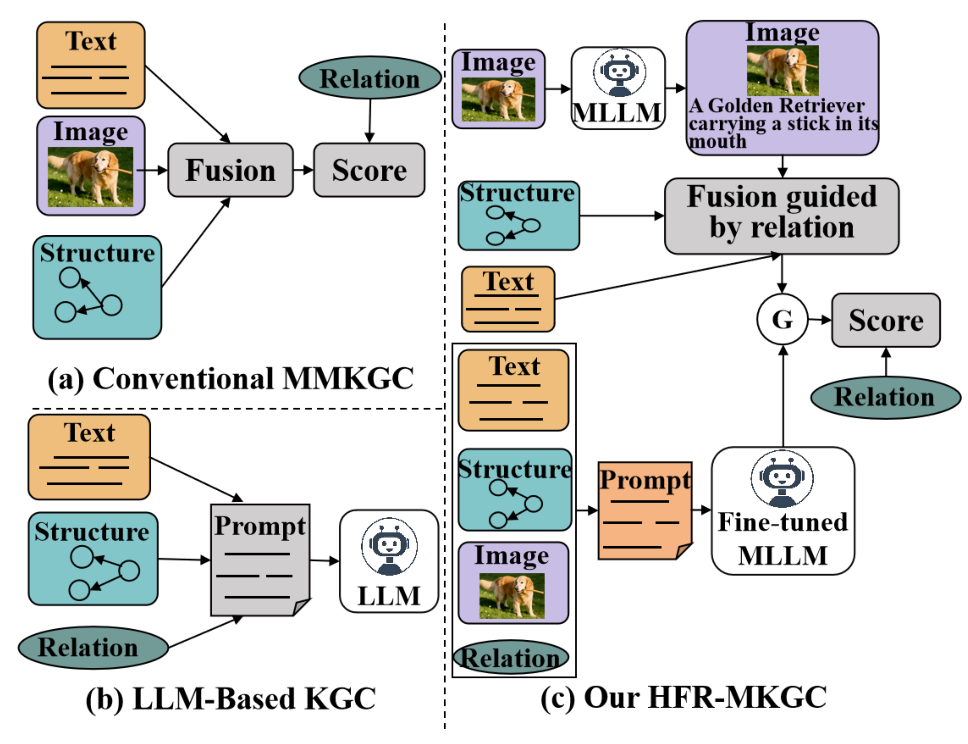
\includegraphics[width=0.8\linewidth]{fig1.png}
\caption{Ba paradigm: (a) MMKGC truyền thống, encoder $\rightarrow$ fusion $\rightarrow$ score; (b) LLM-based KGC, KG $\rightarrow$ prompt $\rightarrow$ LLM; (c) HFR-MKGC kết hợp cả hai. Nguồn: Figure~1 trong~\cite{hfr}, tr.~2.}
\label{fig:paradigm}
\end{figure}

%======================================================================
\section{Các nghiên cứu liên quan (tr.~2)}
%======================================================================

\subsection{MMKGC: ba thế hệ phương pháp trộn mô thức}

\begin{table}[H]
\centering\small
\begin{tabular}{@{}p{2.8cm}p{6.2cm}p{5.4cm}@{}}
\toprule
Nhóm & Đại diện & Ý tưởng\\
\midrule
Early fusion đơn giản & IKRL (Xie 2017), TransAE (Wang 2019), Mousselly-Sergieh 2018 & Nối hoặc cộng trung bình embedding, hoặc autoencoder chung\\
Attention / gating & MKGformer (Chen 2022), RSME~\cite{rsme}, MCKGC (Gao 2025) & Học trọng số trộn nhưng vẫn không phụ thuộc quan hệ\\
Negative sample / adversarial & MACO (Zhang 2023), AdaMF-MAT (Zhang 2024), NativE~\cite{native}, SNAG, DHNS (Chen 2025), APKGC (Jian 2025), MyGO (Zhang 2025) & Sinh mẫu âm khó để tăng tổng quát hoá. Nhóm baseline mạnh nhất; NativE là best baseline của bài\\
\bottomrule
\end{tabular}
\end{table}

Khoảng trống: hầu hết đều relation-agnostic. HFR-MKGC đưa quan hệ vào trọng số trộn.

\subsection{LLM cho suy luận tri thức trên KG}

\begin{itemize}
\item Chuyển cấu trúc KG sang text cho LLM: entity alignment (Jiang 2024, AutoAlign 2023), KGC (KoPA, Zhang 2024; Yao 2025).
\item LP-DIXIT (Barile 2025): dùng LLM đánh giá giải thích link prediction.
\item LoLLM (Pan 2025): LLM kết hợp structure embedding cho KG thưa.
\item MMKG + LLM: UniMEL (Liu 2024) cho entity linking; MuKDC (Li 2024) cho few-shot KGC; CATS (Li 2025) cho inductive KGC.
\end{itemize}

Khoảng trống: LLM-based mới dùng text và cấu trúc, trộn tĩnh. HFR-MKGC dùng MLLM (có ảnh) và cổng động theo từng bộ ba.

%======================================================================
\section{Phương pháp đề xuất HFR-MKGC (tr.~3--5)}
%======================================================================

\subsection{Tổng quan kiến trúc}

Nói ngắn: \textbf{HFR-MKGC = RotatE + trộn đa mô thức có quan hệ dẫn hướng + LLaVA fine-tune + hard negative đối kháng.} Với một query $(h, r, ?)$, mô hình thực hiện ba việc (Hình~\ref{fig:arch}):
\begin{itemize}
\item \textbf{Module 1, RHF}: biến ba vector $(S, I, T)$ của thực thể thành một vector chung $\Hj$, với trọng số tính từ quan hệ $r$.
\item \textbf{Module 2, MER}: LLaVA fine-tune đọc prompt (text, láng giềng, ảnh, $r$) và đoán thẳng tên thực thể thiếu; đáp án được trộn qua cổng vào embedding tail rồi chấm điểm RotatE.
\item \textbf{Module 3, MNO}: tạo hard negative bằng cách bóp méo đặc trưng text (LLaVA viết lại) và ảnh (xoay và nhiễu); huấn luyện đối kháng.
\end{itemize}

\begin{figure}[H]
\centering
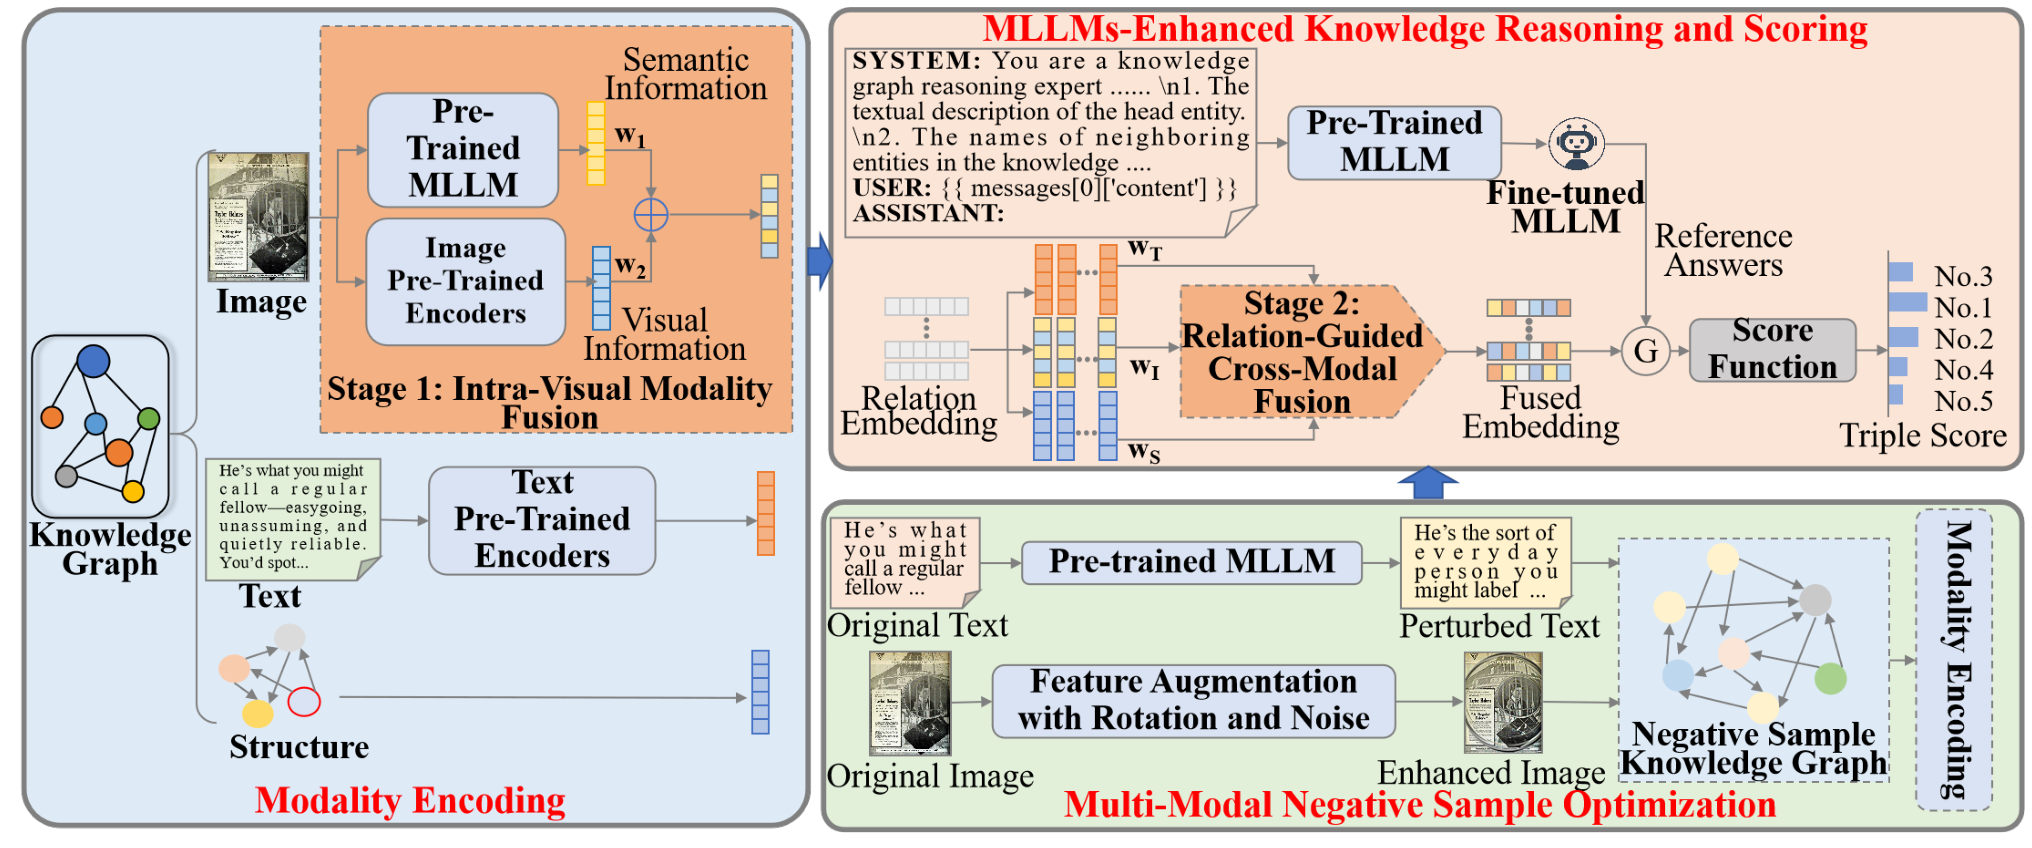
\includegraphics[width=\linewidth]{fig2.png}
\caption{Kiến trúc tổng thể HFR-MKGC. Nguồn: Figure~2 trong~\cite{hfr}, tr.~3.}
\label{fig:arch}
\end{figure}

\begin{table}[H]
\centering\small
\caption{Các mô hình nền được dùng.}
\begin{tabular}{@{}lp{5.6cm}p{6.4cm}@{}}
\toprule
Thành phần & Mô hình & Vai trò\\
\midrule
Encoder ảnh & CLIP~\cite{clip} & ảnh thô $\rightarrow$ vector\\
Encoder text & BERT~\cite{bert} & mô tả text, caption ảnh, đáp án LLaVA $\rightarrow$ vector\\
MLLM & LLaVA-1.5-7B~\cite{llava} + LoRA~\cite{lora} & sinh caption; đoán thực thể thiếu; viết lại text\\
Scoring & RotatE~\cite{rotate} & chấm điểm trong không gian phức\\
Loss & self-adversarial loss của RotatE + adversarial với gradient penalty & huấn luyện\\
\bottomrule
\end{tabular}
\end{table}

\subsection{Mã hoá mô thức (tr.~3)}

Với mỗi thực thể $e$ và mô thức $m \in \{S, I, T\}$:
\begin{equation*}
\mathbf{e}_m = P_m(\mathbf{f}_m) \in \mathbb{R}^d,
\end{equation*}
trong đó $\mathbf{f}_m$ là đặc trưng thô từ encoder pre-trained (CLIP cho ảnh, BERT cho text; $S$ là embedding học tự do) và $P_m$ là lớp chiếu tuyến tính học được, đưa mọi mô thức về cùng chiều $d$. Caption ảnh do MLLM sinh ra cũng được coi là một dạng text.

\subsection{Module 1: Relation-Guided Hierarchical Modal Fusion (RHF)}

Trộn theo hai tầng: tầng 1 trộn bên trong mô thức ảnh, tầng 2 trộn giữa ba mô thức theo quan hệ.

\subsubsection{Tầng 1: Intra-Visual Modality Fusion (Eq.~1, tr.~3)}

\textbf{Tại sao cần.} Ảnh qua CLIP chỉ cho đặc trưng mức pixel (màu, hình dáng). KG cần ngữ nghĩa: đây là ai, làm gì. Tác giả dùng LLaVA viết caption cho ảnh để ``dịch'' ảnh sang ngôn ngữ mà KG hiểu.

\textbf{Cách chạy.} Ảnh $\rightarrow$ CLIP $\rightarrow$ chiếu $\rightarrow$ $\mathbf{e}_{Iv}$ (vector thị giác thô). Ảnh $\rightarrow$ LLaVA sinh caption $\rightarrow$ BERT $\rightarrow$ chiếu $P_T$ $\rightarrow$ $\mathbf{e}_{Ic}$ (vector ngữ nghĩa). Trộn bằng cổng theo độ tương đồng:
\begin{equation}
\mathbf{e}_I = \sigma\big(\langle \mathbf{e}_{Iv}, \mathbf{e}_{Ic}\rangle\big)\,\mathbf{e}_{Ic} + \Big(1 - \sigma\big(\langle \mathbf{e}_{Iv}, \mathbf{e}_{Ic}\rangle\big)\Big)\,\mathbf{e}_{Iv}.
\label{eq:intra}
\end{equation}

\begin{table}[H]
\centering\small
\begin{tabular}{@{}ll@{}}
\toprule
Thành phần & Ý nghĩa\\
\midrule
$\langle \mathbf{e}_{Iv}, \mathbf{e}_{Ic}\rangle$ & tích vô hướng, đo ảnh thô và caption giống nhau bao nhiêu\\
$\sigma(\cdot)$ & sigmoid, đưa về $[0,1]$ làm trọng số\\
trọng số cao & hai vector nhất quán, tin caption\\
trọng số thấp & caption lệch với ảnh, giữ ảnh thô\\
\bottomrule
\end{tabular}
\end{table}

\textbf{Output.} $\mathbf{e}_I \in \mathbb{R}^d$, vừa có thị giác mức thấp vừa có ngữ nghĩa mức cao.

\subsubsection{Tầng 2: Relation-Guided Cross-Modal Fusion (Eq.~2--4, tr.~3--4)}

Đây là ý tưởng cốt lõi của bài: trọng số trộn $S/I/T$ phụ thuộc vào quan hệ $r$. Input là ba vector $\mathbf{H}_e = \{\mathbf{e}_S, \mathbf{e}_I, \mathbf{e}_T\}$ và vector quan hệ $\mathbf{r} \in \mathbb{R}^d$.

\textbf{Bước 1.} Ma trận tương đồng giữa các mô thức: $A_{ij} = \langle \mathbf{e}_i, \mathbf{e}_j\rangle$, $i, j \in \{S, I, T\}$.

\textbf{Bước 2.} Điểm tương tác có quan hệ cho mỗi mô thức $m$:
\begin{equation}
\alpha_m = \underbrace{\langle \mathbf{e}_m, \mathbf{r}\rangle}_{\text{liên quan đến } r} \;+\; \underbrace{\frac{1}{|\mathcal{M}_e|}\sum_{j \in \mathcal{M}_e} A_{mj}}_{\text{nhất quán với mô thức khác}}.
\label{eq:alpha}
\end{equation}
Số hạng thứ nhất đo mô thức $m$ liên quan đến quan hệ $r$ bao nhiêu (số hạng quan trọng nhất). Số hạng thứ hai đo mô thức $m$ nhất quán với các mô thức khác bao nhiêu (trung bình tương đồng), giúp loại mô thức lạc lõng.

\textbf{Bước 3.} Softmax có trừ trung bình để ổn định số:
\begin{equation}
w_m = \frac{\exp(\alpha_m - \bar{\alpha})}{\sum_{j \in \mathcal{M}_e}\exp(\alpha_j - \bar{\alpha})}, \qquad \bar{\alpha} = \frac{1}{|\mathcal{M}_e|}\sum_{k}\alpha_k.
\label{eq:w}
\end{equation}

\textbf{Bước 4.} Embedding chung:
\begin{equation}
\Hj = \sum_{m \in \mathcal{M}_e} w_m\,\mathbf{e}_m.
\label{eq:joint}
\end{equation}
Làm tương tự cho thực thể tail được $\Tj$.

\textbf{Điểm mấu chốt.} Cùng một thực thể, hỏi quan hệ khác thì $w$ khác. Case study (tr.~7) cho thấy với \Ent{voice type}, $w_T$ cao, $w_I$ thấp, đáp án lên hạng 1.

\subsection{Module 2: MLLMs-Enhanced Knowledge Reasoning and Scoring (MER) (tr.~4)}

\subsubsection{Instruction fine-tuning}

Prompt gồm hai phần:
\begin{itemize}
\item $\Prom_{\mathrm{fix}}$: cố định cho mọi mẫu. Mô tả nhiệm vụ (``bạn là chuyên gia suy luận KG, cho bộ ba thiếu tail, hãy đoán\ldots'') và định dạng đầu ra.
\item $\Prom_{\mathrm{var}}(h, r)$: thay đổi theo bộ ba. Gồm mô tả text của $h$, tập láng giềng của $h$ trong KG, ảnh của $h$, và quan hệ $r$.
\end{itemize}
Nhãn giám sát là tail thật $t$. LLaVA được fine-tune bằng LoRA để giữ khả năng tổng quát, chỉ học thêm ma trận hạng thấp.

\subsubsection{Suy luận (Eq.~5)}

\begin{equation}
\hat{t}_{\mathrm{MLLM}} = \mathrm{MLLM}\big(\Prom_{\mathrm{fix}} \oplus \Prom_{\mathrm{var}}(h, r)\big).
\label{eq:mllm}
\end{equation}
LLaVA trả ra tên thực thể dạng text. Sau đó $\Tm = \mathrm{BERT}(\hat{t}_{\mathrm{MLLM}})$ thành vector. Nếu thiếu head thì xây $\Prom_{\mathrm{var}}(t, r)$ đối xứng.

\subsubsection{Cổng trộn trong không gian phức (Eq.~6--9)}

\textbf{Tại sao cần cổng.} LLaVA có thể đoán đúng, cũng có thể ảo giác. Không thể tin 100\%. Cần một cổng học ``tin LLM bao nhiêu'' cho từng bộ ba, từng chiều.

\textbf{Bước 1.} Quan hệ $\mathbf{r}$ thành số phức đơn vị (cách RotatE biểu diễn quan hệ), $\gamma$ điều chỉnh miền giá trị của pha:
\begin{equation}
\mathbf{r}_C = \cos\!\Big(\frac{\mathbf{r}}{\gamma/\pi}\Big) + i\,\sin\!\Big(\frac{\mathbf{r}}{\gamma/\pi}\Big).
\label{eq:rc}
\end{equation}

\textbf{Bước 2.} Tách $\Tj$ và $\Tm$ thành phần thực $\Re(\cdot)$ và phần ảo $\Im(\cdot)$.

\textbf{Bước 3.} Cổng hai lớp, tính từ dự đoán của LLaVA:
\begin{equation}
\mathbf{g} = \sigma\big(W_2 \tanh(W_1 \Tm + \mathbf{b}_1) + \mathbf{b}_2\big) \in [0,1]^{2d}, \qquad \mathbf{g} = [\mathbf{g}_{re};\ \mathbf{g}_{im}].
\label{eq:gate}
\end{equation}

\textbf{Bước 4.} Nội suy từng phần ($\circ$ là nhân từng phần tử):
\begin{align}
\Re(\Tjt) &= (1 - \mathbf{g}_{re}) \circ \Re(\Tj) + \mathbf{g}_{re} \circ \Re(\Tm),\label{eq:re}\\
\Im(\Tjt) &= (1 - \mathbf{g}_{im}) \circ \Im(\Tj) + \mathbf{g}_{im} \circ \Im(\Tm).\label{eq:im}
\end{align}

\begin{table}[H]
\centering\small
\begin{tabular}{@{}ll@{}}
\toprule
Thành phần & Ý nghĩa\\
\midrule
$\mathbf{g}$ gần 1 & tin LLaVA, lấy nhiều từ $\Tm$\\
$\mathbf{g}$ gần 0 & tin embedding, giữ $\Tj$\\
$\circ$ (nhân từng phần tử) & cổng học theo từng chiều\\
$\mathbf{g}$ tính từ $\Tm$ & cổng học ``độ tin cậy'' của chính đáp án LLaVA\\
\bottomrule
\end{tabular}
\end{table}

\subsubsection{Chấm điểm RotatE (Eq.~10)}

\begin{equation}
\score(h, r, t) = -\big\|\Hjt \circ \mathbf{r}_C - \Tjt\big\|.
\label{eq:score}
\end{equation}
Xoay head theo pha quan hệ; càng gần tail thì khoảng cách càng nhỏ, điểm càng cao. Xếp hạng mọi ứng viên theo điểm này.

\textit{Ghi chú khi đọc:} bài ký hiệu $\Hjt$ cho head nhưng chỉ mô tả cổng cho tail. Nhóm hiểu: head đã biết nên dùng $\Hj$ từ RHF; tail (cần đoán) mới trộn thêm gợi ý của LLaVA.

\subsection{Module 3: Multi-Modal Negative Sample Optimization (MNO) (tr.~4--5)}

\textbf{Khác gì negative thường.} Negative thường thay id thực thể, tạo bộ ba sai về cấu trúc. Bài này giữ nguyên thực thể nhưng bóp méo đặc trưng ảnh và text, tạo mẫu ``gần giống thật'', ép mô hình học biểu diễn bền hơn.

\subsubsection{Nhiễu text bằng LLaVA}

\begin{equation*}
\tilde{\mathbf{e}}^{t}_{\mathrm{pert}} = P_t\big(E_{\mathrm{text}}(\mathrm{MLLM}(x^{t}_{\mathrm{orig}}))\big).
\end{equation*}
Đưa mô tả text gốc vào LLaVA, sinh câu cùng nghĩa nhưng khác cách diễn đạt (paraphrase), qua BERT rồi chiếu.

\subsubsection{Nhiễu ảnh bằng xoay và nhiễu Gaussian (Eq.~11)}

\begin{equation}
\tilde{\mathbf{e}}^{v}_{\mathrm{pert}} = \big((1 - \lambda)\mathbf{I} + \lambda\mathbf{R}\big)\,x^{v}_{\mathrm{orig}} + \boldsymbol{\epsilon}.
\label{eq:vis}
\end{equation}

\begin{table}[H]
\centering\small
\begin{tabular}{@{}lp{10cm}@{}}
\toprule
Thành phần & Ý nghĩa\\
\midrule
$\mathbf{R}$ & ma trận xoay, lấy từ phân rã QR của ma trận hạng thấp ngẫu nhiên (đảm bảo trực giao)\\
$\lambda \in [0,1]$ & cường độ xoay, tăng tuyến tính theo epoch (curriculum: đầu dễ, sau khó)\\
$\boldsymbol{\epsilon} \sim \mathcal{N}(0, \sigma^2 \mathbf{I})$ & nhiễu Gaussian\\
\bottomrule
\end{tabular}
\end{table}

\subsubsection{Ba loại negative}

Từ đặc trưng đã nhiễu tạo $(h^*, r, t)$, $(h, r, t^*)$, $(h^*, r, t^*)$, tức $M = 3$ loại, chấm điểm bằng $\score(\cdot)$.

\subsubsection{Huấn luyện đối kháng (Eq.~12--14, tr.~5)}

\textbf{Loss KGC} (phía discriminator), dạng self-adversarial của RotatE:
\begin{equation}
\mathcal{L}_{\mathrm{kgc}} = -\frac{1}{2N}\sum_{i=1}^{N}\Big(\log\sigma(s_i^+) + \sum_{j=1}^{K} w_i^j \log\sigma(-s_{i,j}^-)\Big), \qquad
w_i^j = \frac{\exp(\tau\, s_{i,j}^-)}{\sum_{k=1}^{K}\exp(\tau\, s_{i,k}^-)}.
\label{eq:lkgc}
\end{equation}
Ở đây $s_i^+$ là điểm bộ ba đúng (muốn cao), $s_{i,j}^-$ là điểm negative thứ $j$ (muốn thấp). Trọng số $w_i^j$ càng lớn khi negative có điểm càng cao (càng khó); $\tau$ chỉnh độ sắc. Negative gồm cả loại thay id ngẫu nhiên và loại đa mô thức ở trên.

\textbf{Loss generator:}
\begin{equation}
\mathcal{L}_g = \frac{1}{M}\sum_{k=1}^{M}\mathbb{E}_{(h,r,t)\sim\mathcal{T}}\big[\max(0,\ c - s_k)\big].
\label{eq:lg}
\end{equation}
Generator (bộ tạo nhiễu text/ảnh) bị phạt khi negative loại $k$ có điểm thấp hơn margin $c$, buộc nó sinh mẫu khó hơn.

\textbf{Tổng thể:}
\begin{equation}
\mathcal{L}_D = \mathcal{L}_{\mathrm{kgc}} + \mu_1\,\mathbb{E}_{\hat{f}\sim P_{\hat{f}}}\Big[\big(\|\nabla_{\hat{f}} D(\hat{f})\|_2 - 1\big)^2\Big], \qquad \mathcal{L}_g \text{ như (\ref{eq:lg})}.
\label{eq:ld}
\end{equation}
$D = \score(\cdot)$ là discriminator; $\hat{f}$ là nội suy giữa embedding thật và giả; số hạng thứ hai là gradient penalty để ổn định huấn luyện. Tối ưu xen kẽ $D$ và $G$.

\textbf{Bằng chứng nó có ích.} Bỏ adversarial (w/o MNO) làm MRR trên MKG-W giảm từ 38,62 xuống 34,01 (Table~3).

%======================================================================
\section{Ví dụ minh hoạ: dữ liệu chạy qua mô hình}
%======================================================================

Ví dụ lấy theo case study của bài (Figure~4, tr.~7). Các giá trị trung gian (caption, trọng số, đáp án LLaVA, giá trị cổng) là minh hoạ do nhóm đặt để làm rõ luồng dữ liệu; bài báo không in các giá trị này.

\paragraph{Input.}
\begin{itemize}
\item Query: (\Ent{Gwen Stefani}, \Ent{voice type}, ?).
\item Text của $h$: ``Gwen Renée Stefani (born October 3, 1969) is an American singer, songwriter, actress, and \ldots''
\item Ảnh của $h$: ảnh chân dung Gwen Stefani.
\item Láng giềng của $h$: (\Ent{member of}, \Ent{No Doubt}), (\Ent{place of birth}, \Ent{Anaheim}), \ldots
\item Ứng viên: toàn bộ 15\,000 thực thể trong MKG-W.
\end{itemize}

\paragraph{Bước 1. Mã hoá và trộn (RHF) cho head.}
Ảnh $\rightarrow$ CLIP $\rightarrow$ $\mathbf{e}_{Iv}$. Ảnh $\rightarrow$ LLaVA caption ``a blonde woman singing on stage'' $\rightarrow$ BERT $\rightarrow$ $\mathbf{e}_{Ic}$. $\mathbf{e}_I$ = trộn hai vector bằng cổng tương đồng (\ref{eq:intra}). Text $\rightarrow$ BERT $\rightarrow$ $\mathbf{e}_T$; cấu trúc $\rightarrow$ $\mathbf{e}_S$. Quan hệ \Ent{voice type} $\rightarrow$ $\mathbf{r}$. Theo (\ref{eq:alpha}), $\alpha_T$ cao (text nói ``singer'', liên quan \Ent{voice type}), $\alpha_I$ thấp (ảnh chỉ có ngoại hình), nên $w \approx (S{:}\,0{,}35;\ I{:}\,0{,}15;\ T{:}\,0{,}50)$ và
$\Hj = 0{,}35\,\mathbf{e}_S + 0{,}15\,\mathbf{e}_I + 0{,}50\,\mathbf{e}_T$.

\paragraph{Bước 2. Suy luận bằng LLaVA (MER).}
Prompt $= \Prom_{\mathrm{fix}}$ + [text của $h$, láng giềng, ảnh, ``voice type'']. LLaVA (LoRA) $\rightarrow$ ``Mezzo-soprano'' $\rightarrow$ BERT $\rightarrow$ $\Tm$. Cổng $\mathbf{g}$ = mạng hai lớp($\Tm$), ví dụ trung bình $0{,}6$ (tin LLaVA khá nhiều).

\paragraph{Bước 3. Chấm điểm từng ứng viên $t$.}
$\Tj(t)$ = RHF của ứng viên $t$; $\Tjt(t) = (1-\mathbf{g}) \circ \Tj(t) + \mathbf{g} \circ \Tm$; $\score(t) = -\|\Hj \circ \mathbf{r}_C - \Tjt(t)\|$.

\paragraph{Output (xếp hạng theo score).}
\begin{center}\small
\begin{tabular}{@{}ll@{}}
\toprule
Hạng & Thực thể\\
\midrule
1 & \Ent{Mezzo-soprano} (đáp án đúng)\\
2 & \Ent{Double bass}\\
3 & \Ent{Soprano}\\
\ldots & \ldots\\
\bottomrule
\end{tabular}
\end{center}
Metric cho query này: rank $= 1$, reciprocal rank $= 1{,}0$, Hits@1 $= 1$.

\paragraph{So sánh khi bỏ RHF (theo Figure~4).}
Trọng số không theo quan hệ, ảnh chiếm cao nhất: hạng 1 \Ent{Double bass}, hạng 2 \Ent{Mezzo-soprano}, reciprocal rank $= 0{,}5$.

\paragraph{Khi huấn luyện (MNO).}
Thêm vào mỗi bộ ba đúng các negative: thay id, ví dụ (\Ent{Gwen Stefani}, \Ent{voice type}, \Ent{Anaheim}); đa mô thức $(h^*, r, t)$ với text của $h$ bị LLaVA viết lại thành ``She is a US-born vocalist and composer\ldots'' và vector ảnh bị xoay cộng nhiễu. Discriminator (score) học cho negative điểm thấp; generator học làm negative khó hơn.

%======================================================================
\section{Thực nghiệm (tr.~5--7)}
%======================================================================

\subsection{Dữ liệu (Table~2, tr.~6)}

\begin{table}[H]
\centering\small
\caption{Thống kê ba benchmark.}
\label{tab:data}
\begin{tabular}{@{}llrrrrrrr@{}}
\toprule
Dataset & Nguồn & \#Ent & \#Rel & \#Train & \#Valid & \#Test & \#Image & \#Text\\
\midrule
MKG-W & Xu 2022~\cite{mkg} (Wikidata) & 15\,000 & 169 & 34\,196 & 4\,276 & 4\,274 & 14\,463 & 14\,123\\
MKG-Y & Xu 2022~\cite{mkg} (YAGO) & 15\,000 & 28 & 21\,310 & 2\,665 & 2\,663 & 14\,244 & 12\,305\\
DB15K & Liu 2019~\cite{mmkg} (DBpedia) & 12\,842 & 279 & 79\,222 & 9\,902 & 9\,904 & 12\,818 & 9\,078\\
\bottomrule
\end{tabular}
\end{table}

\textit{Nhận xét của nhóm (suy từ bảng):}
\begin{itemize}
\item Chia xấp xỉ 80/10/10 ở cả ba tập.
\item Không phải thực thể nào cũng đủ ảnh/text. DB15K chỉ khoảng 71\% thực thể có text, MKG-Y khoảng 82\%. Vì thế trộn mô thức phải chịu được thiếu và nhiễu.
\item MKG-Y chỉ có 28 quan hệ, mỗi quan hệ dày, cấu trúc đã đủ mạnh (RotatE thuần đạt 36,67 MRR).
\item DB15K nhiều quan hệ và nhiều bộ ba nhất, đồ thị dày nhất.
\end{itemize}

Định dạng file trong \texttt{original/data/} (copy từ repo MDBGF, cùng benchmark): các file \texttt{train.txt}, \texttt{valid.txt}, \texttt{test.txt} mỗi dòng ``head\_id relation\_id tail\_id''; \texttt{entities.txt} và \texttt{relations.txt} là danh sách id; \texttt{entity2id.txt} ánh xạ tên sang id. Ảnh và text gốc không nằm trong folder.

\subsection{Độ đo và baseline}

Với mỗi bộ ba test, che tail (và che head), chấm điểm toàn bộ thực thể, xem đáp án thật đứng hạng mấy.
\begin{itemize}
\item \textbf{MRR}: trung bình $1/\mathrm{rank}$. Hạng 1 $\rightarrow 1{,}0$, hạng 2 $\rightarrow 0{,}5$, hạng 10 $\rightarrow 0{,}1$.
\item \textbf{Hits@1}: \% đáp án đúng ở hạng 1. Khó nhất.
\item \textbf{Hits@3}: \% đáp án đúng trong top 3.
\item \textbf{Hits@10}: \% đáp án đúng trong top 10. Đo khả năng không bỏ sót.
\end{itemize}
Tất cả tính theo \%, càng cao càng tốt.

14 baseline chia ba nhóm (tr.~5): (1) uni-modal: TransE, RotatE~\cite{rotate}, DistMult, ComplEx; (2) MMKGC: IKRL, RSME~\cite{rsme}, MyGO, NativE~\cite{native}, AdaMF-MAT, SNAG, DHNS, APKGC; (3) MLLM-based: LLaMA-2-7B (prompt có text và láng giềng), LLaVA-1.5-7B~\cite{llava} (thêm ảnh). Hai mô hình cuối chỉ sinh danh sách 10 ứng viên nên không tính được MRR. Tất cả baseline được tái hiện với cùng encoder CLIP/BERT để so sánh công bằng (tr.~6).

\subsection{Thiết lập huấn luyện (tr.~5--6)}

PyTorch, 2 GPU NVIDIA RTX A6000 (48GB), 250 epoch, Adam. Chiều embedding $d \in \{128, 256, 512\}$; số negative mỗi bộ ba $\in \{32, 64, 128\}$; learning rate $\in \{10^{-5}, 10^{-4}, 10^{-3}\}$; batch size $\in \{128, 256, 1024\}$. Chi tiết prompt, số epoch LoRA, cách chọn láng giềng đưa vào prompt không được mô tả.

\subsection{Kết quả chính (Table~1, tr.~6)}

\begin{table}[H]
\centering\footnotesize
\caption{Kết quả link prediction (\%). Bảng rút gọn các baseline đáng chú ý; bảng đầy đủ 14 baseline trong PDF (TransE, DistMult, ComplEx, IKRL, SNAG, DHNS đều thấp hơn). In đậm là tốt nhất trong cột.}
\label{tab:main}
\setlength{\tabcolsep}{2.6pt}
\resizebox{\linewidth}{!}{%
\begin{tabular}{@{}lrrrrrrrrrrrr@{}}
\toprule
& \multicolumn{4}{c}{MKG-W} & \multicolumn{4}{c}{MKG-Y} & \multicolumn{4}{c}{DB15K}\\
\cmidrule(lr){2-5}\cmidrule(lr){6-9}\cmidrule(lr){10-13}
Model & MRR & H@10 & H@3 & H@1 & MRR & H@10 & H@3 & H@1 & MRR & H@10 & H@3 & H@1\\
\midrule
RotatE & 32.92 & 44.23 & 35.91 & 26.68 & 36.67 & 41.11 & 35.91 & 33.92 & 32.07 & 51.40 & 38.57 & 21.23\\
RSME & 33.41 & 44.31 & 35.80 & 27.59 & 38.03 & 44.02 & 35.80 & 34.28 & 33.72 & 50.39 & 39.23 & \textbf{24.45}\\
MyGO & 33.40 & 44.36 & 35.38 & 27.52 & 30.29 & 42.17 & 35.38 & 23.75 & 32.25 & 48.23 & 35.49 & 24.19\\
AdaMF-MAT & 32.09 & 45.78 & 35.54 & 24.48 & 37.78 & 46.11 & 35.54 & 32.65 & 32.08 & 52.42 & 40.41 & 19.81\\
APKGC & 32.67 & 46.20 & 35.83 & 25.24 & 31.48 & 40.68 & 35.83 & 26.17 & 32.91 & 48.91 & 37.15 & 24.39\\
NativE & 36.79 & 50.28 & 40.47 & 29.36 & 38.34 & 46.24 & 40.47 & 33.49 & 33.59 & 53.77 & 40.67 & 22.11\\
LLaMA-2-7B & -- & 10.20 & 8.73 & 5.62 & -- & 2.29 & 2.03 & 1.35 & -- & 14.14 & 11.87 & 7.15\\
LLaVA-1.5-7B & -- & 26.42 & 22.29 & 15.02 & -- & 3.58 & 2.80 & 1.64 & -- & 15.89 & 13.15 & 8.32\\
\midrule
HFR-MKGC & \textbf{38.62} & \textbf{51.66} & \textbf{42.12} & \textbf{31.37} & \textbf{39.00} & \textbf{47.31} & \textbf{42.12} & \textbf{34.41} & \textbf{35.20} & \textbf{56.41} & \textbf{43.25} & 23.04\\
\bottomrule
\end{tabular}}
\end{table}

\textit{Đọc bảng:}
\begin{itemize}
\item HFR-MKGC đứng đầu 11/12 ô. Ngoại lệ duy nhất là Hits@1 trên DB15K (23,04), thua RSME (24,45), APKGC (24,39) và MyGO (24,19). Bài viết ``SOTA trên mọi metric'', nhóm nêu trung thực ngoại lệ này.
\item Trên MKG-W: hơn NativE $+1{,}83$ MRR, $+2{,}01$ Hits@1, $+1{,}65$ Hits@3, $+1{,}38$ Hits@10.
\item Cải thiện trên MKG-Y nhỏ nhất ($+0{,}66$ MRR): tập ít quan hệ, cấu trúc đã đủ mạnh, đa mô thức thêm ít giá trị.
\item LLM thuần rất kém (Hits@10 dưới 27\%): LLM một mình không thay được hàm chấm điểm có cấu trúc. LLaVA (có ảnh) hơn LLaMA (không ảnh) ở mọi tập, cho thấy ảnh có ích.
\end{itemize}

\subsection{Nghiên cứu loại bỏ trên MKG-W (Table~3, tr.~7)}

\begin{table}[H]
\centering\small
\caption{Ablation trên MKG-W (\%).}
\label{tab:abl}
\begin{tabular}{@{}lrrrrl@{}}
\toprule
Cấu hình & MRR & H@10 & H@3 & H@1 & Bỏ gì\\
\midrule
w/o S & 25.67 & 39.42 & 28.81 & 18.02 & bỏ mô thức cấu trúc\\
w/o T & 29.67 & 45.61 & 34.92 & 21.25 & bỏ text\\
w/o V & 31.16 & 47.39 & 36.10 & 22.09 & bỏ ảnh\\
w/o VT & 31.78 & 47.33 & 36.41 & 23.22 & bỏ caption ảnh do LLaVA sinh\\
w/o RHF & 31.98 & 50.25 & 39.14 & 20.80 & thay trộn theo quan hệ bằng trung bình\\
w/o MER & 33.52 & 50.61 & 39.70 & 23.42 & bỏ suy luận LLaVA\\
w/o PTI & 34.59 & 50.95 & 40.03 & 25.12 & thay nhiễu text/ảnh bằng nhiễu ngẫu nhiên\\
w/o MNO & 34.01 & 50.98 & 40.26 & 24.13 & bỏ adversarial training\\
\midrule
Full & \textbf{38.62} & \textbf{51.66} & \textbf{42.12} & \textbf{31.37} & \\
\bottomrule
\end{tabular}
\end{table}

\textit{Đọc bảng:}
\begin{itemize}
\item Cấu trúc quan trọng nhất: bỏ $S$ mất khoảng 13 MRR. Text quan trọng hơn ảnh (bỏ $T$ mất 9, bỏ $V$ mất 7,5).
\item RHF đóng góp lớn nhất trong bốn module: mất 6,6 MRR, Hits@1 rớt từ 31,4 xuống 20,8, nhưng Hits@10 gần như không đổi. Trộn theo quan hệ chủ yếu giúp xếp đúng hạng 1.
\item MER đóng góp khoảng 5 MRR. Hard negative có nghĩa (PTI) và adversarial (MNO) mỗi thứ khoảng 4 đến 4,6 MRR. Caption ảnh (VT) khoảng 6,8 MRR.
\end{itemize}

\subsection{Độ nhạy siêu tham số (Figure~3, tr.~7)}

Khảo sát chiều embedding $\{128, 256, 512\}$ và số negative $\{32, 64, 128\}$ trên MKG-W, so với RotatE:
\begin{itemize}
\item Chiều 512 cần 128 negative mới đạt 38,62 MRR; với 32 hoặc 64 negative chỉ khoảng 33.
\item Chiều 256 tốt nhất với 64 negative (36,08). Chiều 128 gần như không phụ thuộc số negative (khoảng 36).
\item Thiếu negative thì 256 chiều có thể hơn 512 chiều.
\item MRR và Hits@1 nhạy với siêu tham số, Hits@10 ổn định.
\item RotatE thuần tăng đều theo chiều (10 $\rightarrow$ 25 $\rightarrow$ 33 MRR) và không nhạy với số negative.
\end{itemize}

\subsection{Case study (Figure~4, tr.~7)}

\begin{figure}[H]
\centering
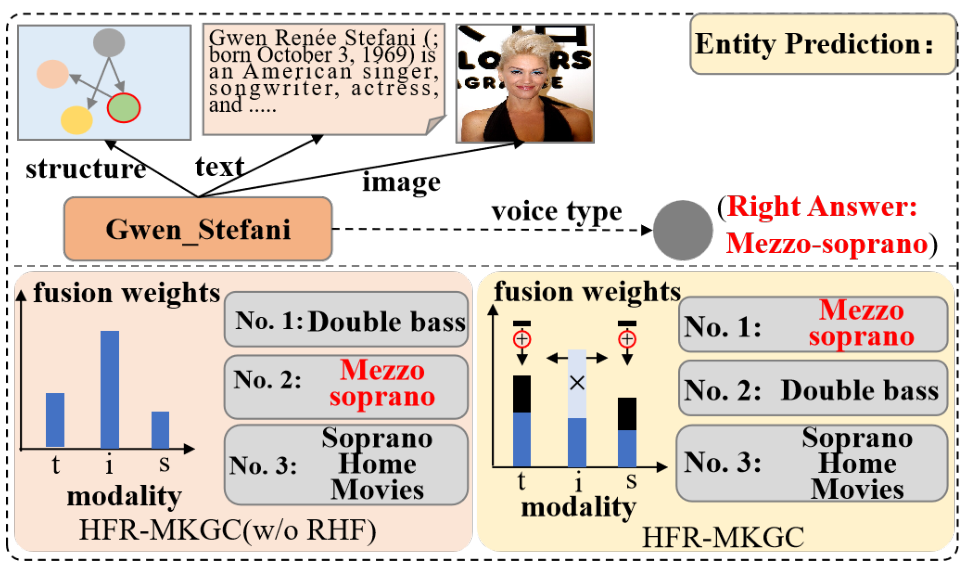
\includegraphics[width=0.75\linewidth]{fig4.png}
\caption{Case study (\Ent{Gwen Stefani}, \Ent{voice type}, ?). Trái: không có RHF, ảnh được trọng số cao nhất, đáp án đúng hạng 2. Phải: có RHF, trọng số text tăng, ảnh giảm, đáp án đúng hạng 1. Nguồn: Figure~4 trong~\cite{hfr}, tr.~7.}
\label{fig:case}
\end{figure}

%======================================================================
\section{Nhận xét và đánh giá của nhóm}
%======================================================================

\subsection{Điểm mạnh}

\begin{itemize}
\item Ý tưởng trọng số trộn phụ thuộc quan hệ đơn giản, có động lực rõ, và ablation cho thấy đây là thành phần đóng góp lớn nhất.
\item Kết hợp được hai paradigm: giữ hàm chấm điểm có cấu trúc (xếp hạng toàn bộ thực thể) nhưng vẫn khai thác được suy luận của MLLM, với cổng học mức tin.
\item Hard negative ở mức đặc trưng là hướng ít được khai thác, và ablation cho thấy hiệu quả hơn nhiễu ngẫu nhiên.
\item Thực nghiệm so sánh với 14 baseline, có ablation, độ nhạy và case study.
\end{itemize}

\subsection{Hạn chế}

\begin{enumerate}
\item \textbf{Chi phí tính toán lớn}: phải chạy LLaVA-7B cho mỗi ảnh (caption), mỗi query (suy luận) và mỗi text (paraphrase). Bài không báo cáo thời gian huấn luyện hay suy luận, cũng không so sánh chi phí với baseline.
\item \textbf{Không có code công khai} (tính đến 2026-09-04 không tìm thấy repo), khó tái lập. Nhiều baseline do tác giả tự tái hiện.
\item \textbf{Cải thiện không đồng đều}: MKG-Y chỉ $+0{,}66$ MRR; thua Hits@1 trên DB15K nhưng bài vẫn tuyên bố SOTA ở mọi metric.
\item \textbf{Ablation chỉ trên MKG-W}, không kiểm tra trên hai tập còn lại.
\item LLaVA chỉ sinh \textbf{một đáp án} $\hat{t}$ rồi BERT-encode. Nếu ảo giác một tên không tồn tại, cổng phải học bỏ qua. Bài không phân tích tỉ lệ LLaVA đoán đúng hay phân bố của cổng $\mathbf{g}$.
\item \textbf{Rò rỉ tri thức tiềm ẩn}: LLaVA và BERT pre-trained trên web có thể đã ``biết'' sự thật trong Wikidata hoặc DBpedia. Bài không thảo luận.
\item Chi tiết prompt, số epoch LoRA, cách chọn láng giềng đưa vào prompt không được mô tả.
\item Ký hiệu đôi chỗ chưa nhất quán ($\Hjt$ chưa định nghĩa; hai tài liệu Chen 2025a/2025b cùng tên ``Noise-powered\ldots'').
\end{enumerate}

\subsection{Câu hỏi thảo luận dự kiến}

\begin{itemize}
\item \textit{Tại sao dùng RotatE mà không phải hàm chấm điểm khác?} RotatE mạnh với quan hệ đối xứng, nghịch đảo, hợp thành; biểu diễn phức thuận tiện cho cổng tách phần thực và phần ảo.
\item \textit{Cổng $\mathbf{g}$ tính từ $\Tm$ chứ không từ $\Tj$, vì sao?} Để cổng học độ tin cậy của chính đáp án LLaVA.
\item \textit{Hard negative đa mô thức khác gì negative thay id?} Thay id tạo bộ ba sai về cấu trúc; đa mô thức giữ nguyên thực thể nhưng bóp méo đặc trưng, ép mô hình học biểu diễn bền hơn.
\item \textit{Mô hình có ngưỡng đúng/sai không?} Không. Link prediction chỉ xếp hạng. Muốn dùng thật phải tự thêm ngưỡng trên validation, thường theo từng quan hệ vì thang điểm RotatE không chuẩn hoá.
\item \textit{Thêm được thực thể mới không?} Không. Mô hình transductive: mỗi thực thể là vector tra bảng học lúc train. Thực thể mới phải train lại. Bài toán đó là inductive KGC (CATS trong related work).
\item \textit{Vì sao LLM thuần kém?} Chỉ sinh 10 ứng viên, không chấm hết tập thực thể; không biết ranh giới tập thực thể; ảo giác.
\item \textit{Caption ảnh có thật sự cần?} Có, bỏ caption (w/o VT) mất khoảng 6,8 MRR.
\end{itemize}

%======================================================================
\section{Kết luận}
%======================================================================

HFR-MKGC~\cite{hfr} giải quyết hai điểm yếu của MMKGC hiện có bằng ba module: (1) RHF trộn phân cấp với trọng số phụ thuộc quan hệ, (2) MER dùng LLaVA fine-tune suy luận theo từng bộ ba và trộn qua cổng vào chấm điểm RotatE, (3) MNO tạo hard negative đa mô thức và huấn luyện đối kháng. Phương pháp đạt kết quả tốt nhất trên 11/12 ô của ba benchmark MKG-W, MKG-Y, DB15K so với 14 baseline; ablation cho thấy trộn theo quan hệ là thành phần đóng góp lớn nhất, chủ yếu ở Hits@1.

Theo nhóm, đóng góp có giá trị nhất của bài là cách kết hợp MLLM vào một hệ thống vẫn xếp hạng toàn bộ thực thể, thay vì để LLM tự trả lời. Hạn chế chính là chi phí tính toán chưa được báo cáo, code không công khai, và một số tuyên bố mạnh hơn số liệu. Hướng tương lai tác giả nêu là khai thác MLLM chính xác hơn cho biểu diễn và suy luận đa mô thức; nhóm cho rằng hướng inductive (thực thể mới) và phân tích độ tin cậy của cổng $\mathbf{g}$ cũng đáng theo đuổi.

%======================================================================
\renewcommand{\refname}{Tài liệu tham khảo (định dạng IEEE)}
\sloppy
\begin{thebibliography}{10}
\small
\bibitem{hfr} D. Wang, J. Du, Z. Xue, M. Liang, G. Ye, Y. Shao, and H. Li, ``HFR-MKGC: Hierarchical Fusion Reasoning with MLLMs for Multi-modal Knowledge Graph Completion,'' in \textit{Proc. AAAI Conf. Artif. Intell.}, vol.~40, no.~18, 2026, pp.~15815--15823. [Online]. Available: \url{https://ojs.aaai.org/index.php/AAAI/article/view/38613}

\bibitem{rotate} Z. Sun, Z.-H. Deng, J.-Y. Nie, and J. Tang, ``RotatE: Knowledge graph embedding by relational rotation in complex space,'' in \textit{Proc. Int. Conf. Learn. Represent. (ICLR)}, 2019.

\bibitem{llava} H. Liu, C. Li, Q. Wu, and Y. J. Lee, ``Visual instruction tuning,'' in \textit{Adv. Neural Inf. Process. Syst. (NeurIPS)}, vol.~36, 2023, pp.~34892--34916.

\bibitem{lora} E. J. Hu, Y. Shen, P. Wallis, Z. Allen-Zhu, Y. Li, S. Wang, L. Wang, and W. Chen, ``LoRA: Low-rank adaptation of large language models,'' in \textit{Proc. Int. Conf. Learn. Represent. (ICLR)}, 2022.

\bibitem{clip} A. Radford \textit{et al.}, ``Learning transferable visual models from natural language supervision,'' in \textit{Proc. Int. Conf. Mach. Learn. (ICML)}, 2021, pp.~8748--8763.

\bibitem{bert} J. Devlin, M.-W. Chang, K. Lee, and K. Toutanova, ``BERT: Pre-training of deep bidirectional transformers for language understanding,'' in \textit{Proc. NAACL-HLT}, 2019, pp.~4171--4186.

\bibitem{mmkg} Y. Liu, H. Li, A. Garcia-Duran, M. Niepert, D. Onoro-Rubio, and D. S. Rosenblum, ``MMKG: Multi-modal knowledge graphs,'' in \textit{Proc. Eur. Semantic Web Conf. (ESWC)}, 2019, pp.~459--474.

\bibitem{mkg} D. Xu, T. Xu, S. Wu, J. Zhou, and E. Chen, ``Relation-enhanced negative sampling for multimodal knowledge graph completion,'' in \textit{Proc. 30th ACM Int. Conf. Multimedia (MM)}, 2022, pp.~3857--3866.

\bibitem{native} Y. Zhang, Z. Chen, L. Guo, Y. Xu, B. Hu, Z. Liu, W. Zhang, and H. Chen, ``NativE: Multi-modal knowledge graph completion in the wild,'' in \textit{Proc. 47th Int. ACM SIGIR Conf. Res. Develop. Inf. Retrieval}, 2024, pp.~91--101.

\bibitem{rsme} M. Wang, S. Wang, H. Yang, Z. Zhang, X. Chen, and G. Qi, ``Is visual context really helpful for knowledge graph? A representation learning perspective,'' in \textit{Proc. 29th ACM Int. Conf. Multimedia (MM)}, 2021, pp.~2735--2743.
\end{thebibliography}

\end{document}
